\documentclass[12pt, letterpaper]{book}

\usepackage{graphicx} %LaTeX package to import graphics
\graphicspath{{images/}} %configuring the graphicx package

\usepackage{amsmath}% For the equation* environment

\setlength{\parskip}{.7em}
\setlength{\parindent}{0pt}

\title{Project Proposal}
\author{Meyer A. Cloete\thanks{sponsored by Hoffies}}
\date{August 2022}

\begin{document}
	\maketitle
	%\begin{abstract}
	%	This is a simple paragraph at the beginning of the 
	%	document. A brief introduction about the main subject.
	%\end{abstract}
	
	After our abstract we can begin the first paragraph, then press ``enter'' twice to start the second one.
	
	This line will start a second paragraph.
	
	I will start the third paragraph and then add \\ a manual line break which causes this text to start on a new line but remains part of the same paragraph. Alternatively, I can use the \verb|\newline|\newline command to start a new line, which is also part of the same paragraph.
	
	Some of the greatest \emph{discoveries} in science 
	were made by accident.
	
	\textit{Some of the greatest \emph{discoveries} in science were made by accident.}
	
	\textbf{Some of the greatest \emph{discoveries} in science were made by accident.}
	
	The universe is immense and it seems to be homogeneous, 
	on a large scale, everywhere we look.
	
	% The \includegraphics command is 
	% provided (implemented) by the 
	% graphicx package
	\begin{figure}[h]
		\centering
		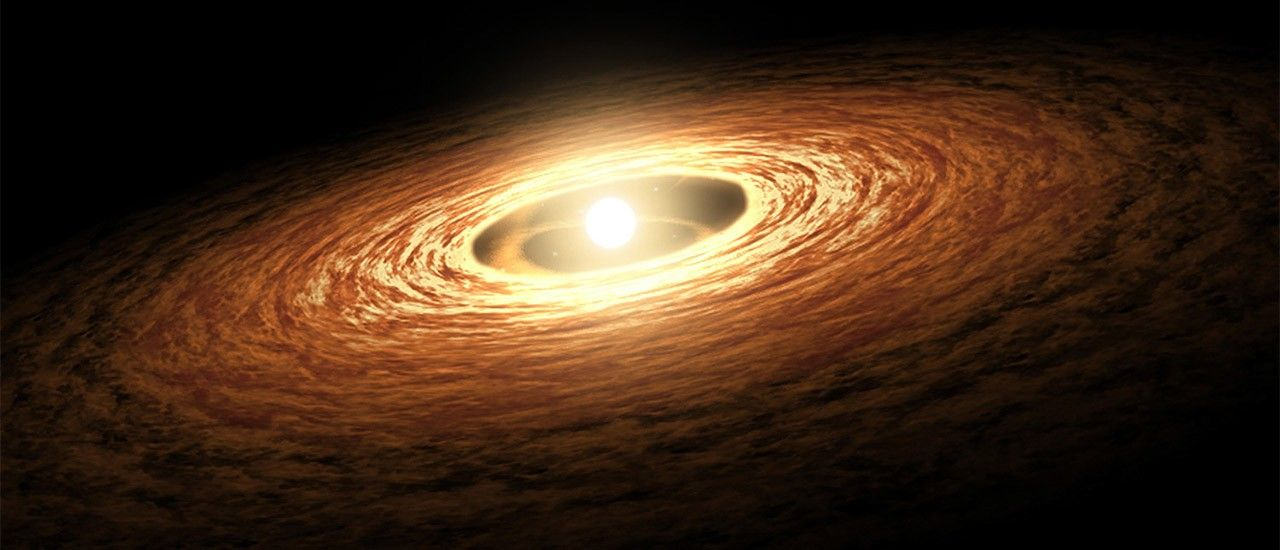
\includegraphics[width=1.2\textwidth]{universe}
		\caption{An Image of an Universe}
	\end{figure} 
	
	A list follows:
	
	\begin{itemize}
		\item The individual entries are indicated with a black dot, a so-called bullet.
		\item The text in the entries may be of any lengthwwwwwwwwwwwwwwwwwwwwwwwwwwwwwwwwwwwwwwwww.
	\end{itemize}
	
	An ordered list follows:
	\begin{enumerate}
		\item This is the first entry in our list.
		\item The list numbers increase with each entry we add.
	\end{enumerate}
	
	In physics, the mass-energy equivalence is stated 
	by the equation $E=mc^2$, discovered in 1905 by Albert Einstein.
	
	Subscripts in math mode are written as $a_b$ and superscripts are written as $a^b$. These can be combined and nested to write expressions such as
	
	\[ T^{i_1 i_2 \dots i_p}_{j_1 j_2 \dots j_q} = T(x^{i_1},\dots,x^{i_p},e_{j_1},\dots,e_{j_q}) \]
	
	We write integrals using $\int$ and fractions using $\frac{a}{b}$. Limits are placed on integrals using superscripts and subscripts:
	
	\[ \int_0^1 \frac{dx}{e^x} =  \frac{e-1}{e} \]
	
	Lower case Greek letters are written as $\omega$ $\delta$ etc. while upper case Greek letters are written as $\Omega$ $\Delta$.
	
	Mathematical operators are prefixed with a backslash as $\sin(\beta)$, $\cos(\alpha)$, $\log(x)$ etc.
	
	\section{First example}
	
	The well-known Pythagorean theorem \(x^2 + y^2 = z^2\) was proved to be invalid for other exponents, meaning the next equation has no integer solutions for \(n>2\):
	
	\[ x^n + y^n = z^n \]
	
	\section{Second example}
	
	This is a simple math expression \(\sqrt{x^2+1}\) inside text. 
	And this is also the same: 
	\begin{math}
		\sqrt{x^2+1}
	\end{math}
	but by using another command.
	
	This is a simple math expression without numbering
	\[\sqrt{x^2+1}\] 
	separated from text.
	
	This is also the same:
	\begin{displaymath}
		\sqrt{x^2+1}
	\end{displaymath}
	
	\ldots and this:
	\begin{equation*}
		\sqrt{x^2+1}
	\end{equation*}
	
	\chapter{First Chapter}
	
	\section{Introduction}
	
	This is the first section.
	
	Lorem  ipsum  dolor  sit  amet,  consectetuer  adipiscing  
	elit. Etiam  lobortisfacilisis sem.  Nullam nec mi et 
	neque pharetra sollicitudin.  Praesent imperdietmi nec ante. 
	Donec ullamcorper, felis non sodales...
	
	\section{Second Section}
	
	Lorem ipsum dolor sit amet, consectetuer adipiscing elit.  
	Etiam lobortis facilisissem.  Nullam nec mi et neque pharetra 
	sollicitudin.  Praesent imperdiet mi necante...
	
	\subsection{First Subsection}
	Praesent imperdietmi nec ante. Donec ullamcorper, felis non sodales...
	
	\section*{Unnumbered Section}
	Lorem ipsum dolor sit amet, consectetuer adipiscing elit.  
	Etiam lobortis facilisissem...
	
	\begin{center}
		\begin{tabular}{c c c}
			cell1 & cell2 & cell3 \\ 
			cell4 & cell5 & cell6 \\  
			cell7 & cell8 & cell9    
		\end{tabular}
	\end{center}
\end{document}